\chapter{热机与机器}\label{ch:b1:heat-engines}

汽车发动机、发电站、冰箱与\omterm{def:b1:heat-engines:machine}{热泵}，
本是从四个角度看到的同一对象：一种流体沿循环走一圈，
轮流与\omterm{def:b1:heat-engines:machine}{热源}和冷源接触，与两者交换热量，
并与轴交换功。第一定律记录能量的收支；
第二定律则通过一个循环上的熵平衡，
给出任何巧妙设计都无法突破的极限——卡诺定理，
这是工程学中最重要的不等式。本章推导这一极限，
计算理想循环，以及趋近它的实际循环（\omterm{prop:b1:heat-engines:otto}{奥托循环}、\omterm{prop:b1:heat-engines:diesel}{狄塞尔循环}、\omterm{prop:b1:heat-engines:stirling}{斯特林循环}），
再把机器反转过来用于制冷与供暖，
并说明实际机器产生的熵，如何一焦耳一焦耳地
以损失的功来“付账”。

\section{循环机器与两条定律}

\begin{definition}[热机]\label{def:b1:heat-engines:machine}
\index{热机}\index{制冷机}\index{热泵}\index{热源}
称\emph{热机}为一个\omterm{def:b1:newton-dynamics:conservation}{封闭系统}（工作物质），
沿\emph{循环}经历一圈，使其周期性地回到同一状态，
同时与外界交换功 $W$，并与热源交换热量 $Q_i$，
这些热源的温度为 $T_i$，称为\emph{热源}，
其温度不因交换热量而改变。\emph{双热源}机器使用两个热源：
高温热源的温度为 $T_h$，低温热源的温度为 $T_c < T_h$。
若机器对外输出功（$W < 0$），则为\emph{热机}；
若机器被驱动（$W > 0$）从冷源吸热，则为\emph{制冷机}；
若被驱动向热源放热，则为\emph{热泵}。
所有量都按一个循环、以\omterm{rem:b1:mirrors-thin-lenses:why}{代数量}计，
即按工作物质所接收的量计算。
\end{definition}

\begin{theorem}[循环上的两条定律；克劳修斯不等式]\label{thm:b1:heat-engines:clausius}
\index{克劳修斯不等式}
对双\omterm{def:b1:heat-engines:machine}{热源}机器的一个循环，
\[
W + Q_h + Q_c = 0 , \qquad
\frac{Q_h}{T_h} + \frac{Q_c}{T_c} = -S_{\text{产生}} \leq 0 ,
\]
第二式中的等号成立，当且仅当该循环是
可逆的。更一般地，对任意多个\omterm{def:b1:heat-engines:machine}{热源}，
$\sum_i Q_i/T_i \leq 0$（\emph{克劳修斯不等式}）。
\end{theorem}

\begin{proof}
$U$ 与 $S$ 都是状态函数，故 $\Delta U = 0$，$\Delta S = 0$ 在
一个循环上成立。由第一定律得 $0 = W + Q_h + Q_c$，由熵平衡
（\cref{thm:b1:second-law-entropy:secondlaw}）得 $0 = S_{\text{交换}} +
S_{\text{产生}}$，其中 $S_{\text{交换}} = \sum Q_i/T_i$，因为每个
\omterm{def:b1:heat-engines:machine}{热源}都在自身固定温度下交换热量
（\cref{prop:b1:second-law-entropy:thermostat}）。
\end{proof}

\begin{corollary}[再论开尔文]\label{cor:b1:heat-engines:kelvin}
\emph{单\omterm{def:b1:heat-engines:machine}{热源}}机器（$Q_c = 0$）满足 $Q_h \leq 0$，从而 $W \geq 0$：
任何循环都不能把单一\omterm{def:b1:heat-engines:machine}{热源}的热量全部转化为功。
船不能靠冷却海水而航行——\omterm{def:b1:heat-engines:machine}{热机}需要冷源
来排出热量，而第二定律说明了必须排出多少。
\end{corollary}

\begin{omfigure}
\begin{tikzpicture}[font=\small, x=1cm, y=1cm, >=Stealth]
  % engine
  \begin{scope}
    \draw[fill=omThm!15, draw=omThm, thick] (-1.6,3.0) rectangle (1.6,3.7) node[midway] {高温热源 $T_h$};
    \draw[fill=omDef!15, draw=omDef, thick] (-1.6,-0.7) rectangle (1.6,0) node[midway] {低温热源 $T_c$};
    \draw[thick, rounded corners, fill=omProp!10] (-0.9,1.0) rectangle (0.9,2.0) node[midway] {热机};
    \draw[->, omThm, very thick] (0,3.0) -- (0,2.0) node[midway, right] {$Q_h > 0$};
    \draw[->, omDef, very thick] (0,1.0) -- (0,0) node[midway, right] {$Q_c < 0$};
    \draw[->, omProp, very thick] (0.9,1.5) -- (2.3,1.5) node[midway, above] {$W < 0$};
    \node[font=\footnotesize] at (0,-1.1) {$\eta = -W/Q_h$};
  \end{scope}
  % refrigerator / heat pump
  \begin{scope}[xshift=6.4cm]
    \draw[fill=omThm!15, draw=omThm, thick] (-1.6,3.0) rectangle (1.6,3.7) node[midway] {高温热源 $T_h$};
    \draw[fill=omDef!15, draw=omDef, thick] (-1.6,-0.7) rectangle (1.6,0) node[midway] {低温热源 $T_c$};
    \draw[thick, rounded corners, fill=omProp!10] (-1.1,1.0) rectangle (1.1,2.0) node[midway, align=center, font=\footnotesize] {制冷机 \\ 或热泵};
    \draw[->, omThm, very thick] (0,2.0) -- (0,3.0) node[midway, right] {$Q_h < 0$};
    \draw[->, omDef, very thick] (0,0) -- (0,1.0) node[midway, right] {$Q_c > 0$};
    \draw[->, omProp, very thick] (-2.5,1.5) -- (-1.1,1.5) node[midway, above] {$W > 0$};
    \node[font=\footnotesize] at (0,-1.1) {$e_f = Q_c/W$, \quad $e_p = -Q_h/W$};
  \end{scope}
\end{tikzpicture}

{\small 双\omterm{def:b1:heat-engines:machine}{热源}循环的两种走向。左：\omterm{def:b1:heat-engines:machine}{热机}从高温\omterm{def:b1:heat-engines:machine}{热源}吸热，
将其中一部分排给低温\omterm{def:b1:heat-engines:machine}{热源}，并把两者之差作为功输出。
右：同一机器反向驱动，把热量由冷源泵向\omterm{def:b1:heat-engines:machine}{热源}；
若需要的是 $Q_c$，则它为\omterm{def:b1:heat-engines:machine}{制冷机}，
若需要的是 $|Q_h|$，则它为\omterm{def:b1:heat-engines:machine}{热泵}。}
\end{omfigure}

\section{卡诺定理}

\begin{definition}[效率与性能系数]\label{def:b1:heat-engines:efficiency}
\index{效率!热机}\index{性能系数}
\omterm{def:b1:heat-engines:machine}{热机}的\emph{效率}是每从高温\omterm{def:b1:heat-engines:machine}{热源}吸取单位热量
所输出的功，即 $\eta = -W/Q_h$；\omterm{def:b1:heat-engines:machine}{制冷机}的\emph{性能系数}（COP）是
每单位功所制取的冷量，即 $e_f = Q_c/W$；\omterm{def:b1:heat-engines:machine}{热泵}的性能系数是
每单位功所供出的热量，即 $e_p = -Q_h/W$。
每个量都是“所要的”与“所付的”之比；
效率至多为~1，
性能系数则可以超过~1。
\end{definition}

\begin{theorem}[卡诺]\label{thm:b1:heat-engines:carnot}
\index{卡诺定理}\index{卡诺效率}
在两\omterm{def:b1:heat-engines:machine}{热源}（$T_h > T_c$）之间，
\[
\eta \leq \eta_C = 1 - \frac{T_c}{T_h}, \qquad
e_f \leq \frac{T_c}{T_h - T_c}, \qquad
e_p \leq \frac{T_h}{T_h - T_c} = 1 + \frac{T_c}{T_h - T_c},
\]
当且仅当循环可逆时取等号。这些界仅依赖于
温度，与工作物质和具体机构无关。
\end{theorem}

\begin{proof}
对\omterm{def:b1:heat-engines:machine}{热机}（$Q_h > 0$）：$\eta = -W/Q_h = (Q_h + Q_c)/Q_h = 1 + Q_c/Q_h$，
由克劳修斯不等式得 $Q_c/Q_h \leq -T_c/T_h$。对
\omterm{def:b1:heat-engines:machine}{制冷机}（$Q_c > 0$，$W > 0$）：$W = -Q_h - Q_c$，且 $-Q_h \geq Q_c T_h/T_c$，
于是 $W \geq Q_c(T_h/T_c - 1)$，且 $e_f = Q_c/W \leq T_c/(T_h - T_c)$。
对\omterm{def:b1:heat-engines:machine}{热泵}，$e_p = -Q_h/W = (W + Q_c)/W = 1 + e_f$。取等号即为
全过程可逆的情形，亦即 $S_{\text{产生}} = 0$。
\end{proof}

\begin{example}[三个数]\label{ex:b1:heat-engines:numbers}
一台蒸汽轮机工作在 $T_h = \qty{800}{K}$ 的\omterm{def:b1:heat-engines:machine}{热源}与
$T_c = \qty{300}{K}$ 的河水之间：$\eta_C = 0.625$；实际电厂约为 $0.40$。
一台家用冰箱工作于内部 $\qty{275}{K}$ 与
$\qty{298}{K}$ 的厨房之间：$e_f \leq 275/23 = 12$；实际机器给出 $2$ 到 $4$。一
台\omterm{def:b1:heat-engines:machine}{热泵}为 $\qty{293}{K}$ 的房屋供暖，取热自 $\qty{273}{K}$ 的空气：
$e_p \leq 293/20 = 14.7$；实际\omterm{def:b1:heat-engines:machine}{热泵}为 $3$ 到 $5$——仍为同样电能
在\omterm{def:b1:dc-circuits:resistor}{电阻器}中所产生热量的三到五倍
（见\cref{pb:b1:heat-engines:1}）。
\end{example}

\begin{remark}[效率为何不能等于~1]\label{rem:b1:heat-engines:why}
\omterm{def:b1:heat-engines:machine}{热机}随所吸收的热量获得熵 $Q_h/T_h$；功
不带走熵；唯一的出路是排向冷源的热量，
它带走的熵为 $|Q_c|/T_c$。熵不可产生，因此至少须
排出 $Q_h T_c/T_h$ 的热量，其余的部分才是功。
冷源越冷、\omterm{def:b1:heat-engines:machine}{热源}越热，\omterm{def:b1:heat-engines:efficiency}{效率}越高——这正是
冷却塔存在的理由，也是人们追求更耐高温的涡轮叶片的原因。
\end{remark}

\section{卡诺循环}

\begin{definition}[卡诺循环]\label{def:b1:heat-engines:carnotcycle}
\index{卡诺循环}
\emph{卡诺循环}是可逆双\omterm{def:b1:heat-engines:machine}{热源}循环：两条可逆
等温线，分别位于 $T_h$（与高温\omterm{def:b1:heat-engines:machine}{热源}接触）和 $T_c$（与低温\omterm{def:b1:heat-engines:machine}{热源}接触），
由两条可逆绝热支（等熵，
不与任何\omterm{def:b1:heat-engines:machine}{热源}接触）连接。在 $(V, P)$ 平面上顺时针运行时为\omterm{def:b1:heat-engines:machine}{热机}，
逆时针运行时则为\omterm{def:b1:heat-engines:machine}{制冷机}或\omterm{def:b1:heat-engines:machine}{热泵}。在\omterm{def:b1:second-law-entropy:TS}{熵图}中
它是一个矩形。
\end{definition}

\begin{proposition}[理想气体的卡诺循环]\label{prop:b1:heat-engines:carnotgas}
对 $n$ \omterm{def:b1:kinetic-theory:scales}{摩尔}\omterm{def:b1:kinetic-theory:model}{理想气体}，沿 $A \to B$（等温线 $T_h$，
膨胀）、$B \to C$（绝热线）、$C \to D$（等温线 $T_c$，
压缩）、$D \to A$（绝热线）进行循环：
\[
Q_h = nRT_h\ln\frac{V_B}{V_A}, \qquad
Q_c = -nRT_c\ln\frac{V_B}{V_A}, \qquad
\eta = 1 - \frac{T_c}{T_h} ,
\]
这正是卡诺值——对任何可逆双\omterm{def:b1:heat-engines:machine}{热源}循环都必然如此。
\end{proposition}

\begin{proof}
\omterm{prop:b1:first-law:transformations}{等温过程}中 $\Delta U = 0$，故 $Q = -W = nRT\ln(V_{\text{终}}/
V_{\text{初}})$。\omterm{prop:b1:first-law:transformations}{绝热过程}中 $TV^{\gamma-1}$ 为常量：
即 $T_hV_B^{\gamma-1} = T_cV_C^{\gamma-1}$，且 $T_hV_A^{\gamma-1} =
T_cV_D^{\gamma-1}$，由此得 $V_C/V_D = V_B/V_A$，且 $Q_c = nRT_c\ln(V_D/V_C) =
-nRT_c\ln(V_B/V_A)$。于是 $\eta = 1 + Q_c/Q_h = 1 - T_c/T_h$。
\end{proof}

\begin{omfigure}
\begin{tikzpicture}
\begin{axis}[omaxis, axis x line=bottom, axis y line=left, width=7.6cm, height=5.6cm,
    xlabel={$V$}, ylabel={$P$}, xmin=0, xmax=6.3, ymin=0, ymax=1.7,
    xlabel style={at={(axis description cs:0.5,-0.06)}, anchor=north},
    xtick=\empty, ytick=\empty, samples=60]
  \addplot[omThm, thick, domain=1:2] {1.5/x} node[pos=0.5, above right, font=\footnotesize] {$T_h$};
  \addplot[omProp, thick, domain=2:5.51] {0.75*(2/x)^1.4};
  \addplot[omDef, thick, domain=2.756:5.51] {1/x} node[pos=0.2, below left, font=\footnotesize] {$T_c$};
  \addplot[omProp, thick, domain=1:2.756] {0.3628*(2.756/x)^1.4};
  \node[font=\footnotesize, anchor=south west] at (axis cs:0.95,1.52) {$A$};
  \node[font=\footnotesize, anchor=south west] at (axis cs:2.05,0.77) {$B$};
  \node[font=\footnotesize, anchor=north west] at (axis cs:5.5,0.18) {$C$};
  \node[font=\footnotesize, anchor=north east] at (axis cs:2.7,0.35) {$D$};
  \node[font=\footnotesize, omProp] at (axis cs:4.4,0.62) {绝热线};
  \draw[-Stealth, thick] (axis cs:1.45,1.1) -- (axis cs:1.55,1.0);
  \draw[-Stealth, thick] (axis cs:4.3,0.22) -- (axis cs:4.1,0.235);
\end{axis}
\end{tikzpicture}\hfill
\begin{tikzpicture}
\begin{axis}[omaxis, axis x line=bottom, axis y line=left, width=6.2cm, height=5.6cm,
    xlabel={$S$}, ylabel={$T$}, xmin=-1.2, xmax=4.6, ymin=0, ymax=2.2, clip=false,
    xlabel style={at={(axis description cs:0.5,-0.1)}, anchor=north},
    xtick={1,3}, xticklabels={$S_1$,$S_2$}, ytick={0.8,1.6}, yticklabels={$T_c$,$T_h$}]
  \fill[omProp!20] (axis cs:1,0.8) rectangle (axis cs:3,1.6);
  \draw[omThm, thick, -Stealth] (axis cs:1,1.6) -- (axis cs:3,1.6) node[midway, above, font=\footnotesize] {$A \to B$};
  \draw[omProp, thick, -Stealth] (axis cs:3,1.6) -- (axis cs:3,0.8) node[midway, right, font=\footnotesize] {$B \to C$};
  \draw[omDef, thick, -Stealth] (axis cs:3,0.8) -- (axis cs:1,0.8) node[midway, below, font=\footnotesize] {$C \to D$};
  \draw[omProp, thick, -Stealth] (axis cs:1,0.8) -- (axis cs:1,1.6) node[midway, left, font=\footnotesize] {$D \to A$};
  \node[font=\footnotesize] at (axis cs:2,1.2) {$-W$};
\end{axis}
\end{tikzpicture}

{\small \omterm{def:b1:kinetic-theory:model}{理想气体}的\omterm{def:b1:heat-engines:carnotcycle}{卡诺循环}。左图：在克拉珀龙图中，两条等温线与两条
（更陡的）绝热线，沿顺时针方向运行；所围面积即为输出的功。右图：
同一循环在\omterm{def:b1:second-law-entropy:TS}{熵图}中为一个矩形，高为 $T_h - T_c$，宽为
$Q_h/T_h$；其面积同样为 $-W$，该面积与顶边下方的面积 
$Q_h$ 之比，
经观察即为 $1 - T_c/T_h$。}
\end{omfigure}

\begin{remark}[卡诺循环是定理，而非热机]\label{rem:b1:heat-engines:notengine}
可逆\omterm{prop:b1:first-law:transformations}{等温过程}要求热量在温差趋于零的情况下无限缓慢地传递：
卡诺\omterm{def:b1:heat-engines:machine}{热机}以零功率输出其最大功。
实际机器以\omterm{def:b1:heat-engines:efficiency}{效率}换取功率，在换热器中接受有限的
温差，
（见\cref{exo:b1:heat-engines:10}）。卡诺值仍是
一切设计所对照的上限。
\end{remark}

\section{真实热机循环}

\begin{proposition}[奥托循环]\label{prop:b1:heat-engines:otto}
\index{奥托循环}\index{压缩比}
理想化汽油机使空气（$\gamma$）经历如下循环：$1 \to 2$
从 $V_1$ 到 $V_2$ 的绝热压缩（\emph{\omterm{prop:b1:heat-engines:otto}{压缩比}}
$r = V_1/V_2$）；$2 \to 3$ 等容加热（燃烧）；$3 \to 4$
绝\omterm{prop:b1:kinetic-theory:condensed}{热膨胀}回到 $V_1$；$4 \to 1$ 等容降温（
排气）。其\omterm{def:b1:heat-engines:efficiency}{效率}为
\[
\eta_{\text{奥托}} = 1 - \frac{1}{r^{\gamma-1}} .
\]
\end{proposition}

\begin{proof}
仅在等容线上发生热交换：$Q_h = nC_{V,m}(T_3 - T_2)$，且
$Q_c = nC_{V,m}(T_1 - T_4)$。在绝热线上 $TV^{\gamma-1}$ 为常量：
$T_2 = T_1r^{\gamma-1}$，$T_3 = T_4r^{\gamma-1}$，故 $T_3 - T_2 =
(T_4 - T_1)r^{\gamma-1}$，于是
$\eta = 1 + Q_c/Q_h = 1 - (T_4 - T_1)/(T_3 - T_2) = 1 - r^{1-\gamma}$。
\end{proof}

\begin{example}[汽油机的数值]\label{ex:b1:heat-engines:ottonumbers}
$r = 9$，$\gamma = 1.4$：$9^{0.4} = 2.41$，$\eta = 0.58$。实际汽油机
的\omterm{def:b1:heat-engines:efficiency}{效率}约为 $0.30$：燃烧并非瞬时完成，气体
在 \qty{2500}{K} 时并非\omterm{def:b1:kinetic-theory:model}{理想气体}，热量漏向壁面，摩擦与泵气
各占一份。提高 $r$ 有帮助——直到空气与燃料的混合物在压缩末期
自行点燃（爆震）；柴油机
把这一缺陷变为其工作原理。
\end{example}

\begin{proposition}[狄塞尔循环]\label{prop:b1:heat-engines:diesel}
\index{狄塞尔循环}
将\omterm{prop:b1:heat-engines:otto}{奥托循环}中的等容加热换为等压加热，自
$V_2$ 至 $V_3 = \rho V_2$（\emph{截止比} $\rho > 1$）：燃料喷入
已因\omterm{prop:b1:heat-engines:otto}{压缩比} $r$ 为 $15$ 至 $22$ 而升温的空气中，
随即燃烧。于是
\[
\eta_{\text{狄塞尔}} = 1 - \frac{1}{r^{\gamma-1}}\,\frac{\rho^{\gamma} - 1}{\gamma(\rho - 1)} ,
\]
在相同 $r$ 下小于奥托值，但需在大得多的 $r$ 下方能达到，
因而实际上\omterm{def:b1:heat-engines:efficiency}{效率}更高（大型发动机为 $0.40$ 至 $0.45$）。
\end{proposition}

\begin{proof}
$Q_h = nC_{P,m}(T_3 - T_2)$，$Q_c = nC_{V,m}(T_1 - T_4)$，故 $\eta = 1 -
(T_4 - T_1)/[\gamma(T_3 - T_2)]$。由 $T_2 = T_1r^{\gamma-1}$，$T_3 =
\rho T_2$，并由绝热线 $3 \to 4$（$V_4 = V_1 = rV_2$）得 $T_4 =
T_3(V_3/V_4)^{\gamma-1} = \rho T_1 r^{\gamma-1}(\rho/r)^{\gamma-1} = T_1\rho^{\gamma}$：
$\eta = 1 - (\rho^\gamma - 1)/[\gamma r^{\gamma-1}(\rho - 1)]$。
\end{proof}

\begin{omfigure}
\begin{tikzpicture}
\begin{axis}[omaxis, axis x line=bottom, axis y line=left, width=7.2cm, height=5.6cm,
    xlabel={$V$}, ylabel={$P$}, xmin=0, xmax=5.6, ymin=0, ymax=15.5, clip=false,
    xlabel style={at={(axis description cs:0.5,-0.06)}, anchor=north},
    xtick={1,4}, xticklabels={$V_2$,$V_1$}, ytick=\empty, samples=60]
  \addplot[omProp, thick, domain=1:4] {x^(-1.4)*6.96};
  \addplot[omThm, very thick] coordinates {(1,6.96) (1,13.9)};
  \addplot[omProp, thick, domain=1:4] {13.9*x^(-1.4)};
  \addplot[omDef, very thick] coordinates {(4,2.0) (4,1)};
  \node[font=\footnotesize, anchor=north east] at (axis cs:3.95,0.95) {$1$};
  \node[font=\footnotesize, anchor=east] at (axis cs:0.9,6.96) {$2$};
  \node[font=\footnotesize, anchor=south west] at (axis cs:1.05,13.9) {$3$};
  \node[font=\footnotesize, anchor=south west] at (axis cs:4.05,2.1) {$4$};
  \node[font=\footnotesize, omThm, anchor=west] at (axis cs:1.15,10.5) {$Q_h$（燃烧）};
  \node[font=\footnotesize, omDef, anchor=west] at (axis cs:4.15,1.0) {$Q_c$（排气）};
  \draw[-Stealth, thick] (axis cs:2.0,5.25) -- (axis cs:2.2,4.6);
  \draw[-Stealth, thick] (axis cs:2.2,2.33) -- (axis cs:2.0,2.65);
  \node[font=\footnotesize, omProp, anchor=west] (lblexp) at (axis cs:2.9,6.4) {膨胀};
  \draw[omProp, -Stealth] (lblexp.west) -- (axis cs:2.55,3.9);
  \node[font=\footnotesize, omProp, anchor=west] (lblcomp) at (axis cs:4.4,4.6) {压缩};
  \draw[omProp, -Stealth] (lblcomp.west) -- (axis cs:3.3,1.45);
\end{axis}
\end{tikzpicture}\hfill
\begin{tikzpicture}
\begin{axis}[omaxis, axis x line=bottom, axis y line=left, width=6.6cm, height=5.6cm,
    xlabel={$r$}, ylabel={$\eta$}, xmin=0, xmax=22, ymin=0, ymax=1.05,
    xlabel style={at={(axis description cs:0.5,-0.12)}, anchor=north},
    xtick={5,10,15,20}, ytick={0.2,0.4,0.6,0.8,1}, samples=80]
  \addplot[omThm, thick, domain=1:22] {1-x^(-0.4)} node[pos=0.55, above, font=\footnotesize] {奥托，$\gamma = 1.4$};
  \addplot[omDef, thick, domain=1.5:22] {1-(2^1.4-1)/(1.4*x^0.4*(2-1))} node[pos=0.415, below right, font=\footnotesize, align=left] {狄塞尔，\\ $\rho = 2$};
  \addplot[omProp, dashed, thick] coordinates {(9,0) (9,0.585)};
  \addplot[omProp, dashed, thick] coordinates {(18,0) (18,0.632)};
\end{axis}
\end{tikzpicture}

{\small 左图：克拉珀龙图中的\omterm{prop:b1:heat-engines:otto}{奥托循环}（取 $r = 4$）：两条绝热线和两条等容线；
热量在上止点进入，
随排气排出。右图：理想\omterm{def:b1:heat-engines:efficiency}{效率}随\omterm{prop:b1:heat-engines:otto}{压缩比}的变化；
虚线标出汽油机（$r = 9$）与
柴油机（$r = 18$，$\rho = 2$）。}
\end{omfigure}

\begin{proposition}[斯特林循环与回热器]\label{prop:b1:heat-engines:stirling}
\index{斯特林循环}\index{回热器}
两条等温线（$T_c$，$T_h$）由两条等容线相连。等容段的热量
$\pm nC_{V,m}(T_h - T_c)$，二者大小相等、方向相反；若将其
储存于降温段的\emph{\omterm{prop:b1:heat-engines:stirling}{回热器}}（一种供气体流经的多孔物质）中，
并在升温段送回，则只有等温线
与\omterm{def:b1:heat-engines:machine}{热源}交换热量，且 $\eta = 1 - T_c/T_h$：斯特林\omterm{def:b1:heat-engines:machine}{热机}
除循环形状之外，它就是一台卡诺\omterm{def:b1:heat-engines:machine}{热机}。无\omterm{prop:b1:heat-engines:stirling}{回热器}时，
等容段的热量必须取自\omterm{def:b1:heat-engines:machine}{热源}，且
$\eta = \dfrac{nR(T_h - T_c)\ln(V_1/V_2)}{nRT_h\ln(V_1/V_2) + nC_{V,m}(T_h - T_c)}$，
其值明显更小（见\cref{exo:b1:heat-engines:8}）。
\end{proposition}

\begin{proof}
在等温线上 $Q_h = nRT_h\ln(V_1/V_2)$，$Q_c = -nRT_c\ln(V_1/V_2)$，故
$-W = Q_h + Q_c + 0$，待等容段热量相消后，除以各情形下
实际从\omterm{def:b1:heat-engines:machine}{热源}吸取的热量。
\end{proof}

\begin{remark}[蒸汽轮机与燃气轮机]\label{rem:b1:heat-engines:turbines}
电站并不使用气缸中的气体，而是使用煮沸的水，
使其膨胀通过汽轮机，再冷凝并泵回（朗肯循环，
含两次相变——\cref{ch:b1:phase-changes}），或者使用空气：
空气被压缩，经燃烧加热后在燃气轮机中膨胀（布雷顿循环，
含两条绝热线与两条等压线）。它们的分析需要流动流体的能量平衡，
该内容见本科二年级分册；卡诺界与本章的逻辑同样适用，
无需改动。
\end{remark}

\section{制冷机与热泵}

\begin{definition}[蒸气压缩循环]\label{def:b1:heat-engines:vapourcycle}
\index{蒸气压缩循环}\index{制冷剂}
几乎所有冰箱、冷柜、空调和\omterm{def:b1:heat-engines:machine}{热泵}都让
\emph{制冷剂}在四个部件之间循环：\emph{压缩机}
（外界对其做功，提高蒸气的压强）、\emph{冷凝器}
（热蒸气在高压下液化，向热端放出
$|Q_h|$），\emph{膨胀阀}（液体在无功、无热交换的条件下降至低压，
并部分闪蒸为蒸气），以及\emph{蒸发器}（其余液体在低压下沸腾，
从冷端吸收 $Q_c$）。热量以汽化潜热的形式输运，
两个压强分别决定
两个沸腾温度
（\cref{ch:b1:phase-changes}）。
\end{definition}

\begin{omfigure}
\begin{tikzpicture}[font=\small, x=1cm, y=1cm, >=Stealth, box/.style={draw, thick, rounded corners, minimum width=2.3cm, minimum height=0.8cm, align=center}]
  \node[box, fill=omThm!12] (cond) at (0,2.2) {冷凝器 \\ \footnotesize 高 $P$，$T_{\mathrm{cd}}$};
  \node[box, fill=omDef!12] (evap) at (0,-2.2) {蒸发器 \\ \footnotesize 低 $P$，$T_{\mathrm{ev}}$};
  \node[box, fill=omProp!12] (comp) at (3.4,0) {压缩机};
  \node[box, fill=omExo!12] (valve) at (-3.4,0) {膨胀阀};
  \draw[->, thick] (evap.east) -| (comp.south) node[pos=0.75, right, font=\footnotesize] {蒸气};
  \draw[->, thick] (comp.north) |- (cond.east) node[pos=0.25, right, font=\footnotesize] {热蒸气};
  \draw[->, thick] (cond.west) -| (valve.north) node[pos=0.75, left, font=\footnotesize] {液体};
  \draw[->, thick] (valve.south) |- (evap.west) node[pos=0.25, left, font=\footnotesize] {液体 + 蒸气};
  \draw[->, omThm, very thick] (cond.north) -- ++(0,0.8) node[above, font=\footnotesize] {$|Q_h|$ 流向热端（$T_h < T_{\mathrm{cd}}$）};
  \draw[->, omDef, very thick] (0,-3.8) node[below, font=\footnotesize] {$Q_c$ 来自冷端（$T_c > T_{\mathrm{ev}}$）} -- (evap.south);
  \draw[->, omProp, very thick] (5.6,0) node[right, font=\footnotesize] {$W$} -- (comp.east);
\end{tikzpicture}

{\small \omterm{def:b1:heat-engines:vapourcycle}{蒸气压缩循环}。\omterm{def:b1:heat-engines:vapourcycle}{制冷剂}在
蒸发器中沸腾，温度低于冷端；在冷凝器中凝结，
温度高于热端：热量沿自然方向流过每个换热器，
压缩机负责把热量从
$T_{\mathrm{ev}}$ 提升到 $T_{\mathrm{cd}}$。}
\end{omfigure}

\begin{proposition}[温差的代价]\label{prop:b1:heat-engines:gaps}
一台可逆机在其内部温度
$T_{\mathrm{ev}} < T_c$ 与 $T_{\mathrm{cd}} > T_h$ 之间工作，其 $e_p = T_{\mathrm{cd}}/(T_{\mathrm{cd}} - T_{\mathrm{ev}})$，
小于两\omterm{def:b1:heat-engines:machine}{热源}之间的卡诺值；实际机器只能达到
该值的一部分（通常为 $0.4$ 至 $0.6$）。
因此\omterm{def:b1:heat-engines:machine}{热泵}的性能随室外温度降低、
随供暖回路所需温度升高而下降。
\end{proposition}

\begin{proof}
将\cref{thm:b1:heat-engines:carnot}应用于工质，其\omterm{def:b1:heat-engines:machine}{热源}实际上
即为换热器温度，$T_{\mathrm{cd}} - T_{\mathrm{ev}} >
T_h - T_c$ 使比值减小。
\end{proof}

\begin{omfigure}
\begin{tikzpicture}
\begin{axis}[omaxis, axis x line=bottom, axis y line=left, width=10cm, height=7cm,
    xlabel={室外温度（\unit{\degreeCelsius}）}, ylabel={$e_p$},
    xlabel style={at={(axis description cs:0.5,-0.08)}, anchor=north},
    xmin=-21, xmax=16, ymin=0, ymax=16, xtick={-20,-10,0,10}, ytick={2,4,...,14}, samples=80, clip=false]
  \addplot[omThm, thick, domain=-20:1.5] {293/(20-x)};
  \node[omThm, font=\footnotesize, anchor=west] at (axis cs:-20,13.9) {卡诺，室内 / 室外空气};
  \addplot[omDef, thick, domain=-20:15] {313/(321-(273+x))};
  \node[omDef, font=\footnotesize, anchor=south east] at (axis cs:15.5,10.3) {计入换热器温差的卡诺};
  \addplot[omProp, thick, domain=-20:15] {0.55*313/(321-(273+x))};
  \node[omProp, font=\footnotesize, anchor=south west] at (axis cs:-19.5,3.1) {实际机器};
  \addplot[black, dashed] coordinates {(-21,1) (16,1)} node[pos=0.9, above, font=\footnotesize] {电阻器};
\end{axis}
\end{tikzpicture}

{\small \omterm{def:b1:heat-engines:machine}{热泵}的\omterm{def:b1:heat-engines:efficiency}{性能系数}随室外温度的变化：
室内（\qty{20}{\degreeCelsius}）与室外空气之间的卡诺界；
计入换热器温差后的界
（$T_{\mathrm{cd}} = \qty{313}{K}$，$T_{\mathrm{ev}} = T_{\mathrm{out}} - \qty{8}{K}$）；
以及该界的 $0.55$ 倍所对应的实际机器。即使在 \qty{-10}{\degreeCelsius} 时，
实际\omterm{def:b1:heat-engines:machine}{热泵}每消耗一焦耳电能仍可输送约三焦耳热量，
而\omterm{def:b1:dc-circuits:resistor}{电阻器}只能给出一焦耳。}
\end{omfigure}

\begin{example}[热泵还是电阻？]\label{ex:b1:heat-engines:hpvsresistor}
室外 \qty{-5}{\degreeCelsius} 时，一座房屋散热的功率为 \qty{6}{kW}，
若用\omterm{def:b1:dc-circuits:resistor}{电阻器}供暖，需要 \qty{6}{kW} 的\omterm{thm:b1:dc-circuits:kirchhoff}{电功率}；理想\omterm{def:b1:heat-engines:machine}{热泵}从
\qty{268}{K} 至 \qty{293}{K}，需要 $6/11.7 = \qty{0.51}{kW}$；实际机器
的换热器温度为 \qty{260}{K} 与 \qty{313}{K}，
\omterm{def:b1:transient-regimes:secondorder}{品质因数}为 $0.55$，$e_p = 0.55 \times 313/53 = 3.2$，需要 \qty{1.9}{kW}。
周末问题将整个供暖季节算清，包括熵的影响。
\end{example}

\section{熵与损失功}

\begin{theorem}[损失功]\label{thm:b1:heat-engines:lostwork}
\index{损失功}
一台双\omterm{def:b1:heat-engines:machine}{热源}\omterm{def:b1:heat-engines:machine}{热机}每循环产生熵 $S_{\text{产生}}$，
输出的功为
\[
-W = Q_h\Bigl(1 - \frac{T_c}{T_h}\Bigr) - T_c\,S_{\text{产生}} ,
\]
一台双\omterm{def:b1:heat-engines:machine}{热源}\omterm{def:b1:heat-engines:machine}{热泵}输送 $|Q_h|$，则消耗
$W = |Q_h|(1 - T_c/T_h) + T_c\,S_{\text{产生}}$：每产生一焦耳每\omterm{def:b1:kinetic-theory:temperature}{开尔文}的熵，
就需耗费 $T_c$ 焦耳的功；冷源温度即为
熵与功之间的交换率。
\end{theorem}

\begin{proof}
由\cref{thm:b1:heat-engines:clausius}可得 $Q_c = -T_c(Q_h/T_h + S_{\text{产生}})$；
代入 $-W = Q_h + Q_c$。对\omterm{def:b1:heat-engines:machine}{热泵}，
取 $Q_h < 0$，写出相同的两个关系式。
\end{proof}

\begin{method}[热机的审计]\label{meth:b1:heat-engines:audit}
测量（或计算）与各\omterm{def:b1:heat-engines:machine}{热源}交换的热量及功；
检验热力学第一定律；计算每循环的 $S_{\text{产生}} = -\sum Q_i/T_i$，
或每秒的值；\omterm{thm:b1:heat-engines:lostwork}{损失功}率为 $T_c\dot S_{\text{产生}}$；定位熵产生的
来源（换热器中有限温差、摩擦、节流及非准静态压缩），
通过依次对每个部件应用熵平衡。
不产生熵的部件，
不值得改进。
\end{method}

\begin{example}[一座电站的审计]\label{ex:b1:heat-engines:audit}
\omterm{def:b1:heat-engines:machine}{热源}温度 \qty{800}{K}，河水温度 \qty{300}{K}，输出\omterm{thm:b1:dc-circuits:kirchhoff}{电功率} $\qty{1.0}{GW}$，
\omterm{def:b1:heat-engines:efficiency}{效率} $\eta = 0.40$：$\dot Q_h = \qty{2.5}{GW}$，$\dot Q_c = \qty{1.5}{GW}$，于是
$\dot S_{\text{产生}} = 1.5/300 - 2.5/800 = \qty{1.9}{MW/K}$，损失的
功率为 $300 \times 1.9 = \qty{0.56}{GW}$，恰好等于
卡诺输出 $0.625 \times 2.5 = \qty{1.56}{GW}$ 与实际的 \qty{1.0}{GW} 之差。
河水因需带走的 \qty{1.5}{GW} 热量而升温；夏季河水温热而水量偏少时，
电厂便要降低出力。
\end{example}

\section{练习}

\begin{exercise}[$\star$]\label{exo:b1:heat-engines:1}
一座电站在 \qty{800}{K} 处吸热，
向 \qty{300}{K} 的河流放热。求\omterm{thm:b1:heat-engines:carnot}{卡诺效率}；若实际\omterm{def:b1:heat-engines:efficiency}{效率}为 $0.40$，
\omterm{thm:b1:dc-circuits:kirchhoff}{电功率}输出为 \qty{1.0}{GW}，求每秒从燃料吸取的热量，
以及每秒排入河流的热量。
\end{exercise}

\begin{exercise}[$\star$]\label{exo:b1:heat-engines:2}
一台冰箱把内部保持在 \qty{275}{K}，置于
\qty{298}{K} 的厨房中。求最大\omterm{def:b1:heat-engines:efficiency}{性能系数}；若实际\omterm{def:b1:heat-engines:efficiency}{性能系数}为 $3$，
求抵消经墙壁漏入的 \qty{100}{W} 热量
所需的\omterm{thm:b1:dc-circuits:kirchhoff}{电功率}。
\end{exercise}

\begin{exercise}[$\star$]\label{exo:b1:heat-engines:3}
求 $r = 9$、$\gamma = 1.4$ 的\omterm{prop:b1:heat-engines:otto}{奥托循环}理想\omterm{def:b1:heat-engines:efficiency}{效率}；若取
$r = 11$（现代直喷发动机），其\omterm{def:b1:heat-engines:efficiency}{效率}如何？为何不取 $r = 20$？
\end{exercise}

\begin{exercise}[$\star$]\label{exo:b1:heat-engines:4}
一台\omterm{def:b1:heat-engines:machine}{热泵}从 \qty{280}{K} 的室外空气中取热，为温度 \qty{300}{K} 的房屋供暖。
求最大 $e_p$；供暖需求为 \qty{5}{kW} 时，
理想\omterm{def:b1:heat-engines:machine}{热泵}与实际 $e_p = 3.5$ 的\omterm{def:b1:heat-engines:machine}{热泵}所需\omterm{thm:b1:dc-circuits:kirchhoff}{电功率}分别为多少；
并与\omterm{def:b1:dc-circuits:resistor}{电阻器}作比较。
\end{exercise}

\begin{exercise}[$\star\star$]\label{exo:b1:heat-engines:5}
一\omterm{def:b1:kinetic-theory:scales}{摩尔}\omterm{def:b1:kinetic-theory:model}{理想气体}（$\gamma = 1.4$）在
$T_h = \qty{500}{K}$ 与 $T_c = \qty{300}{K}$ 之间作\omterm{def:b1:heat-engines:carnotcycle}{卡诺循环}；高温\omterm{prop:b1:first-law:transformations}{等温过程}使其
从 \qty{1.0}{L} 变到 \qty{3.0}{L}。求 $V_C$、$V_D$、$Q_h$、$Q_c$、$W$，
并检验\omterm{def:b1:heat-engines:efficiency}{效率}。
\end{exercise}

\begin{exercise}[$\star\star$]\label{exo:b1:heat-engines:6}
某发明者声称一台循环机器每循环从
\qty{400}{K} 的\omterm{def:b1:heat-engines:machine}{热源}吸热 \qty{1000}{J}，向 \qty{300}{K} 的\omterm{def:b1:heat-engines:machine}{热源}放出 \qty{800}{J}，
并输出 \qty{200}{J} 的功。是否可能？求每循环产生的熵。
另一位发明者声称从同样的
\qty{1000}{J} 中获得 \qty{300}{J} 的功，放出 \qty{700}{J}。是否可能？
从这 \qty{1000}{J} 中最多能获得多少功？
\end{exercise}

\begin{exercise}[$\star\star$]\label{exo:b1:heat-engines:7}
求 $r = 18$、$\rho = 2$、$\gamma = 1.4$ 的柴油循环\omterm{def:b1:heat-engines:efficiency}{效率}；
与相同 $r$ 的\omterm{prop:b1:heat-engines:otto}{奥托循环}，以及
$r = 9$ 时的\omterm{prop:b1:heat-engines:otto}{奥托循环}作比较。为何柴油机可以采用如此大的 $r$？
\end{exercise}

\begin{exercise}[$\star\star$]\label{exo:b1:heat-engines:8}
一\omterm{def:b1:kinetic-theory:scales}{摩尔}\omterm{prop:b1:kinetic-theory:Ugas}{双原子气体}（$C_{V,m} = \tfrac52R$）在
\qty{600}{K} 与 \qty{300}{K} 之间进行\omterm{prop:b1:heat-engines:stirling}{斯特林循环}，体积比 $V_1/V_2 = 2$。求每循环的
功；求有理想\omterm{prop:b1:heat-engines:stirling}{回热器}及无\omterm{prop:b1:heat-engines:stirling}{回热器}时的\omterm{def:b1:heat-engines:efficiency}{效率}。
\end{exercise}

\begin{exercise}[$\star\star$]\label{exo:b1:heat-engines:9}
两块相同的物块，热容均为 $C = \qty{4.0}{kJ/K}$，初温分别为 $T_1 =
\qty{400}{K}$ 与 $T_2 = \qty{300}{K}$，用作某\omterm{def:b1:heat-engines:machine}{热机}的\omterm{def:b1:heat-engines:machine}{热源}，
直至达到共同温度 $T_f$。证明可逆\omterm{def:b1:heat-engines:machine}{热机}可获得最大功，
此时 $T_f = \sqrt{T_1T_2}$，并
求 $W_{\max}$。若将两物块简单接触，则 $T_f$ 为多少，
此时产生多少熵？
\end{exercise}

\begin{exercise}[$\star\star\star$]\label{exo:b1:heat-engines:10}
\emph{最大功率下的\omterm{def:b1:heat-engines:machine}{热机}。}一台可逆\omterm{def:b1:heat-engines:machine}{热机}在
内部温度 $x$ 与 $y$ 之间工作，并通过电导为 $K$ 的热交换器交换热量，
即 $\dot Q_h = K(T_h - x)$ 与
$|\dot Q_c| = K(y - T_c)$。(a) 写出功率 $P$ 及
可逆核心的熵条件。(b) 证明 $y = xT_c/(2x - T_h)$，
且 $P = \frac{K}{2}\bigl[(T_h + T_c) - u - T_hT_c/u\bigr]$，其中 $u = 2x - T_h$。
(c) 关于 $u$ 求最大值，证明最大功率下的\omterm{def:b1:heat-engines:efficiency}{效率}为
$\eta^\ast = 1 - \sqrt{T_c/T_h}$。(d) 取 $T_h = \qty{800}{K}$，
$T_c = \qty{300}{K}$ 计算数值，并与\cref{exo:b1:heat-engines:1}比较。
\end{exercise}

\begin{exercise}[$\star\star\star$]\label{exo:b1:heat-engines:11}
\emph{吸收式\omterm{def:b1:heat-engines:machine}{制冷机}。}一台无运动部件的机器
从燃烧器吸取热量 $Q_h$，燃烧器温度为 $T_h$，
从冷室吸取热量 $Q_c$，冷室温度为 $T_c$，并向温度为 $T_0$ 的房间放热（$T_c < T_0 <
T_h$），不做功。证明
$Q_c/Q_h \leq \bigl(1 - T_0/T_h\bigr)\,T_c/(T_0 - T_c)$，并解释
这两个因子的含义，并计算 $T_h = \qty{400}{K}$，$T_0 =
\qty{300}{K}$，$T_c = \qty{275}{K}$ 时该上界的值。
\end{exercise}

\begin{exercise}[$\star\star\star$]\label{exo:b1:heat-engines:12}
\emph{用电供暖，分三种方式。}电能由\omterm{def:b1:heat-engines:efficiency}{效率}为
$0.40$ 的火电站发出。每焦耳燃料热量，
有多少热量能到达住宅：(a) 经\omterm{def:b1:dc-circuits:resistor}{电阻器}，(b) 经
\omterm{def:b1:heat-engines:machine}{热泵}（$e_p = 3.5$），(c) 若燃料直接在\omterm{def:b1:heat-engines:efficiency}{效率}为
$0.90$ 的锅炉中燃烧？(d) 理想情形：可逆\omterm{def:b1:heat-engines:machine}{热机}工作于
\qty{800}{K} 与 \qty{293}{K} 之间的可逆\omterm{def:b1:heat-engines:machine}{热机}驱动
工作于 \qty{273}{K} 与 \qty{293}{K} 之间的可逆\omterm{def:b1:heat-engines:machine}{热泵}——每焦耳燃料可得多少热量，以及
为何结果大于 1 而不与任何规律相矛盾？
\end{exercise}

\begin{omfigure}
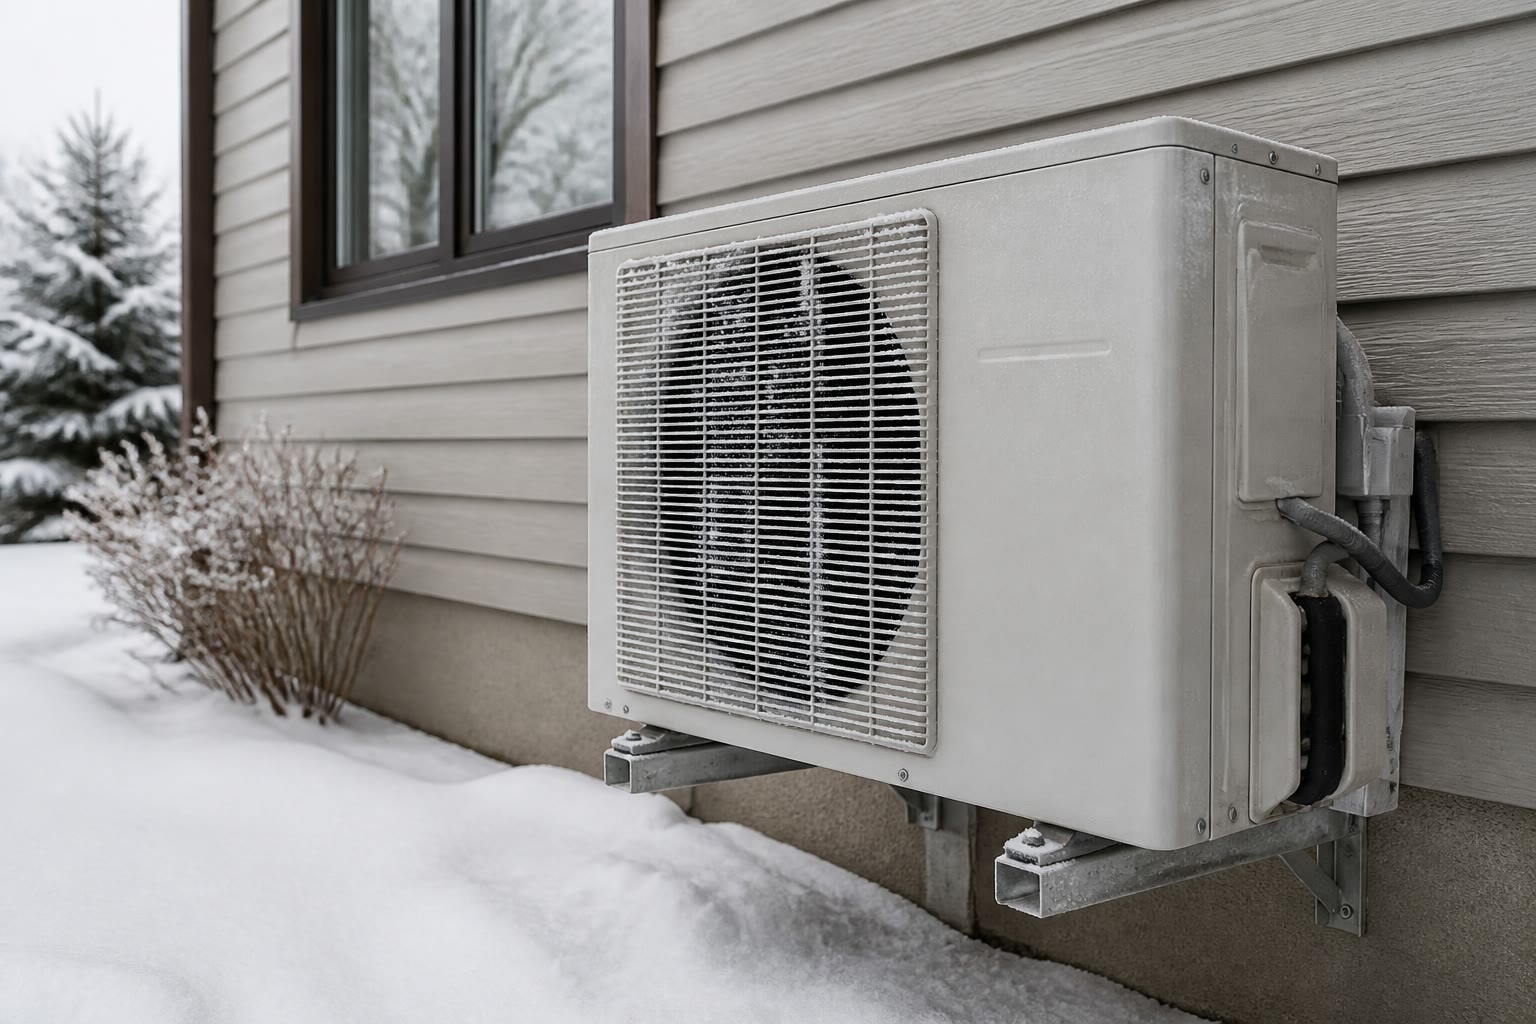
\includegraphics[width=0.58\linewidth]{images/book3/ai/b3-24-heat-pump-winter.jpg}

{\small 冬季的空气源\omterm{def:b1:heat-engines:machine}{热泵}：从寒冷的室外空气吸取热量，向房屋供应的能量为其耗电量的三至四倍——周末问题。}
\end{omfigure}

\section{问题：房屋热泵}

\begin{problem}[{周末问题——冬季房屋供暖：
分别用电阻、燃气、理想热泵和实际热泵供暖时的账单，以及
实际热泵的电能去向何处}]
\label{pb:b1:heat-engines:1}
房屋以 $K(T_{\mathrm{in}} - T_{\mathrm{out}})$ 的速率散热，其中
$K = \qty{250}{W/K}$；室内保持在 $T_{\mathrm{in}} = \qty{20}{\degreeCelsius}$。
设计室外温度为 $\qty{-5}{\degreeCelsius}$；供暖季：
$200$ 天，平均室外温度为 \qty{7}{\degreeCelsius}。
价格：电价 0.25~\texteuro{} 每 \unit{kW h}，燃气 0.10~\texteuro{} 每
\unit{kW h}；$\qty{1}{kW h} = \qty{3.6}{MJ}$。

\medskip
\noindent\textbf{第一部分——房屋与传统供暖方式。}
\begin{enumerate}
  \item 设计温度下所需的供暖功率。
  \item 整个供暖季所需的能量，分别以焦耳和 \unit{kW h} 表示。
  \item 使用\omterm{def:b1:dc-circuits:resistor}{电阻器}供暖的季节费用。
  \item \omterm{def:b1:heat-engines:efficiency}{效率}为 $0.90$ 的燃气锅炉供暖的费用。
  \item 电能来自\omterm{def:b1:heat-engines:efficiency}{效率}为
        $0.40$ 的火电站。\omterm{def:b1:dc-circuits:resistor}{电阻器}与锅炉在一个供暖季中消耗的燃料能量，
        分别为多少；评论“电加热在热力学上是
        浪费的”。
\end{enumerate}

\medskip
\noindent\textbf{第二部分——理想\omterm{def:b1:heat-engines:machine}{热泵}。}
\begin{enumerate}[resume]
  \item 定义 $e_p$，并由热力学两条定律对一个循环证明
        $e_p \leq T_{\mathrm{in}}/(T_{\mathrm{in}} - T_{\mathrm{out}})$。
  \item 设计温度下的理想 $e_p$，以及此时所需的
        \omterm{thm:b1:dc-circuits:kirchhoff}{电功率}。
  \item 供暖季平均温度下的理想 $e_p$，并
        取该值代表整个供暖季，求季节耗电量。
  \item 从物理上解释室外温度降低时 $e_p$ 为何下降，
        以及为何这是供暖装置可能出现的
        最糟糕的性能。
  \item 在设计点，理想\omterm{def:b1:heat-engines:machine}{热泵}耗电 \qty{0.53}{kW}，并
        供热 \qty{6.25}{kW}：其余的 \qty{5.7}{kW} 来自何处，
        以及为何将寒冷的室外空气降温以加热温暖的房屋
        并不违反热力学第二定律？
\end{enumerate}

\medskip
\noindent\textbf{第三部分——实际机器。}
\omterm{def:b1:heat-engines:machine}{热泵}运行\omterm{def:b1:heat-engines:vapourcycle}{蒸气压缩循环}，\omterm{def:b1:heat-engines:vapourcycle}{制冷剂}在
$T_{\mathrm{ev}} = T_{\mathrm{out}} - \qty{8}{K}$ 下蒸发，并在
$T_{\mathrm{cd}} = \qty{313}{K}$ 下冷凝（地暖回路的水温为
\qty{35}{\degreeCelsius}）；机器的性能为卡诺值的 $0.55$ 倍，
该卡诺值按 $T_{\mathrm{ev}}$ 与 $T_{\mathrm{cd}}$ 之间计算。\omterm{def:b1:heat-engines:vapourcycle}{制冷剂}的潜热为
$L = \qty{200}{kJ/kg}$。
\begin{enumerate}[resume]
  \item 写出循环的四个部件，并说明流体在哪个部件中
        吸收 $Q_c$、放出 $|Q_h|$、接收 $W$，以及为何
        蒸发器必须比室外空气更冷，冷凝器
        必须比房屋更热。
  \item 设计温度下的 $T_{\mathrm{ev}}$，以及卡诺 $e_p$
        （在 $T_{\mathrm{ev}}$ 与 $T_{\mathrm{cd}}$ 之间计算）。
  \item 设计温度下的实际 $e_p$、所耗\omterm{thm:b1:dc-circuits:kirchhoff}{电功率}，以及
        从室外空气吸取的热量。
  \item 流经蒸发器的\omterm{def:b1:heat-engines:vapourcycle}{制冷剂}质量流量。
  \item 同样的问题（实际 $e_p$、所耗\omterm{thm:b1:dc-circuits:kirchhoff}{电功率}），针对
        平均温度 \qty{7}{\degreeCelsius}，此时房屋散热
        功率为 \qty{3.25}{kW}。
  \item 将 $e_p$ 表示为 $T_{\mathrm{out}}$ 的函数；
        求季节耗电量与费用，取平均温度下的 $e_p$ 作整个供暖季的值。
        与第一部分比较。
  \item \omterm{def:b1:heat-engines:machine}{热泵}供暖季中火电站所消耗的燃料能量，
        并与\omterm{def:b1:dc-circuits:resistor}{电阻器}及锅炉方案比较。
  \item 在 \qty{-15}{\degreeCelsius} 的寒潮中：热需求、实际 $e_p$、
        若\omterm{def:b1:heat-engines:machine}{热泵}能够供应此热量时的\omterm{thm:b1:dc-circuits:kirchhoff}{电功率}。压缩机的
        制热能力实际上随 $T_{\mathrm{ev}}$ 下降，此时\omterm{def:b1:heat-engines:machine}{热泵}只能
        供热 \qty{3.8}{kW}：所需的备用\omterm{def:b1:dc-circuits:resistor}{电阻器}功率，以及
        “\omterm{def:b1:heat-engines:machine}{热泵}选型”的含义。
  \item 若房屋的旧式散热器需要温度为
        \qty{60}{\degreeCelsius} 的热水（$T_{\mathrm{cd}} = \qty{338}{K}$），求设计温度下的实际 $e_p$
        与所耗\omterm{thm:b1:dc-circuits:kirchhoff}{电功率}，并就
        散热器的选择作出结论。
\end{enumerate}

\medskip
\noindent\textbf{第四部分——电能去向何处。}
\begin{enumerate}[resume]
  \item 证明：对于向房屋输送热量 $|Q_h|$、温度为 $T_{\mathrm{in}}$ 的\omterm{def:b1:heat-engines:machine}{热泵}，
        其取自温度为 $T_{\mathrm{out}}$ 的室外空气，
        $W = |Q_h|(1 - T_{\mathrm{out}}/T_{\mathrm{in}}) + T_{\mathrm{out}}S_{\text{产生}}$ 成立。
  \item 在设计点，每秒钟由热传递产生的熵，
        分别计算冷凝器（自 \qty{313}{K} 到房屋）与
        蒸发器（自室外空气到 \qty{260}{K}）中的值。
  \item 这两处温差所耗费的\omterm{thm:b1:dc-circuits:kirchhoff}{电功率}，及其占
        所耗 \qty{1.92}{kW} 的比例。
  \item 实际机器每秒产生的熵总量（将其
        \qty{1.92}{kW} 与理想情形的 \qty{0.53}{kW} 相比较）；换热器所占的
        份额，并指出其他来源。
  \item 将两处温差减半（\qty{4}{K} 与 \qty{10}{K}），换热器中产生的熵
        及节省的\omterm{thm:b1:dc-circuits:kirchhoff}{电功率}；将温差减半，设计者需付出
        什么代价？
  \item 用三个数值作总结：供暖季中每千瓦时电能对应的供热量（以千瓦时计）；
        季节费用与燃气供暖相比的结果；以及
        电力每
        \unit{kW h} 排放 \qty{60}{g} 的 CO$_2$，燃气按 \qty{200}{g} 计，求各途径
        排放的碳量。
\end{enumerate}
\end{problem}
